\documentclass[12pt]{article}

\usepackage[margin=1in]{geometry}

\usepackage{amsmath, graphicx, caption, subcaption, xcolor}

\graphicspath{{res/}}

% I need a punchy title which is general enough
% to fit all three (if I can pull them off) points from the lab manual.
\title{\textcolor{red}{The Galactic Plane}}

\author{Lukas Finkbeiner}

\begin{document}

\maketitle

\begin{abstract}

We study

1. velocity patterns of various H clouds using Doppler shifts

2. black hole mass

3. accuracy of a spiral arm fit

results, uncertainties.

\end{abstract}

\section{Introduction and Background}

% However, I have not yet actually incorporated equation 8 into my analysis.
\begin{equation}
want two fit equations from the lab manual, eq.s 1 and 8
\end{equation}

We also want gain / calibration equations from lab 2.

Given certain patterns, how well does a spiral fit? We need to control for the total number of data. We want the normalization of any two compared sets to be the same (so, we scale accordingly). What numpy functions I used.

I definitely want to describe the Leuschner dish, some features in the signal chain, maybe just borrow the whole image and edit from there.

\section{Methods}

\quad \quad To observe the galactic plane, we have our trusty tracking script. After three labs' worth of development, it is almost correct!

We convert from galactic to topocentric coordinates using rotation matrices, as described in a previous report. How much should I include? If I describe the matrices again, that will certainly have to go in the introduction.

We probably want a basic run-down of a .fits file, but perhaps some of that can go in the introduction.

The Leuschner dish did not automatically report the frequency axis, \textcolor{red}{I think}. I should describe how I went from .fits file to calibrated spectrum (this includes determining the frequency axis).

%\begin{figure}
%	\centering
%	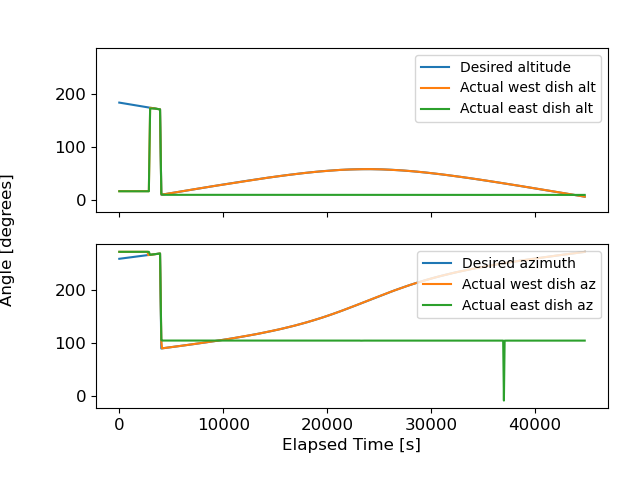
\includegraphics[width=.6\linewidth]{lockup}
%	\caption{These are the comparisons between the input dish angles (as computed with rotation matrices) and the true angles as reported by the dishes. The east dish displays little to no response, indicating that it was stuck for the virtually the entire capture.}
%	\label{fig:stuck}
%\end{figure}

\section{Observations}

\quad \quad What would be a good $introduction$ to the data? We have hundreds of raw spectra. I am not sure how to $succinctly$ describe observations before we get into the analysis.

\section{Analysis}

\quad \quad I should explain how I am going from a spectrum to a point on our galactic plane map. 

\begin{equation} \label{eq:fringes_expect}
f_f = \left[ 800 \cos \delta \right] \cos h_{s, 0} \times \frac{2 \pi}{60 \times 60 \times 24} \approx \frac{\cos \delta \cos h_{s, 0}}{17.19}
\end{equation} 

The recording of the Sun ran from 9:03:19 am to 10:07:02 am on Thursday 3/12. We define the meridian to be $h_s = 0$, and a full solar day to be $2\pi$ radians. Then, we find that the hour angle ranges, approximately, from $-0.7709$ to $-0.4888$. This allows us to construct a plot of, as a function of time, the expected and observed fringe frequencies of the Sun (figure \ref{fig:Sun_fringes}). We see that the percent error is as large as ten percent with the first observation, but that the model and observations seem to agree at greater values of time. Alternatively, one can see there is perhaps a dip in discrepancies around the center, which suggests that the null contributes to the narrowing of error.

\begin{figure}
	\centering
	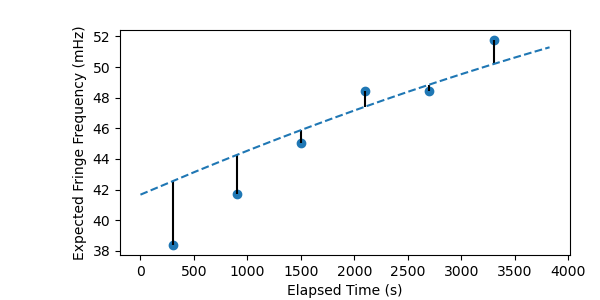
\includegraphics[width=.6\linewidth]{yeah_thatsright}
	\caption{A plot of the fringe frequencies calculated by ten-minute windows in the Sun data. The dashed line represents the values we would expect, based on equation \ref{eq:fringes_expect}.}
	\label{fig:Sun_fringes}
\end{figure}

We largely disregard our results for the Moon and Cygnus A, but we add, as an interesting note, our plots for observed fringe frequencies. They potentially speak about the effectiveness of a single interferometer. However, I could not guess as to how a single interferometer could recover useful data if the interferometer by construction multiplies the two antannae's signals together, and one antenna points to what we can mathematically approximate as, on average, a random patch of the sky. 

Figure \ref{fig:Moon_fringes} shows a patchy trend of the fringe frequency moving up and then down over the course of the whole capture. This would agree with our model. Figure \ref{fig:CygA_fringes} is less consistent. We would expect that the fringe frequency of a point source does not change much as it traverses the sky, so it is at least reassuring that the plot lacks a clear pattern (perhaps representing noise around a point). These plots were independently verified at several places, to make sure that the fringe calculator was operating appropriately.

\begin{figure}
	\centering
	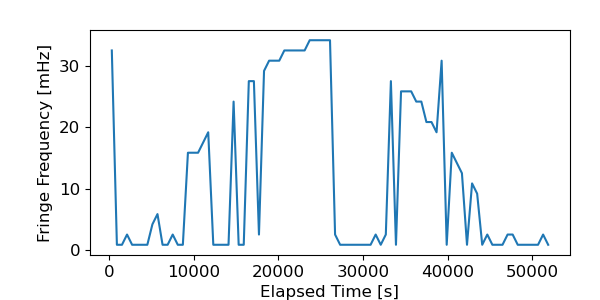
\includegraphics[width=.6\linewidth]{fringes/Moon_fringe}
	\caption{A plot of the fringe frequencies calculated by ten-minute windows in the Moon data. We see that only the largest dip (near 30000 seconds) corresponds to the raw data (figure \ref{fig:Moon_envelope}). Consequently, only so much information can be salvaged.}
	\label{fig:Moon_fringes}
\end{figure}

\begin{figure}
	\centering
	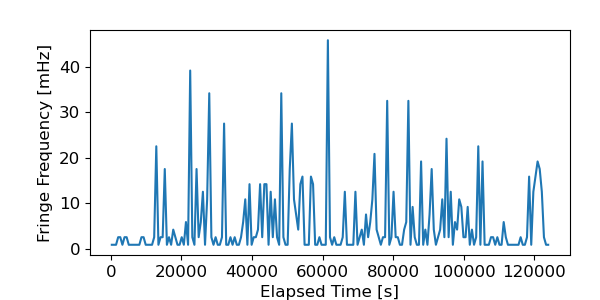
\includegraphics[width=.6\linewidth]{fringes/Cyg_fringe}
	\caption{A plot of the fringe frequencies calculated by ten-minute windows of the Cygnus A data. We see a sporadic pattern of spikes of varying magnitudes; it is less clear that there is a salvageable picture from these data.}
	\label{fig:CygA_fringes}
\end{figure}

\section{Conclusions}

\quad \quad Perhaps the single greatest obstacle to our data collection turned out to be the freezing of the antennae (which our group found not to resolve itself even over a horizon-to-horizon capture). Initially, we had written the script to automatically raise an exception whenever there was a discrepancy of greater than one fifth of a degree between the just-repositioned antennae's self-reported angles and the angles that we had requested. For reasons still unknown, the script kept raising exceptions even when my parallel inquiries showed that the antennae did in fact agree. In any case, we failed to procure, on time, a script that would automatically detect antennae freezing.
 
Therefore, the situation called for the manual spotting of antenna failures. However, this raises its own set of issues. Even with the latest version of our data-taking script, the failure of a dish can take a while to show up in the data. Consider the magnitudes along the x-axis of figure \ref{fig:stuck}. Consider, especially, how the gap closed between the azimuths of the two antennae from about 5000 to 10000 seconds. That is a span of about an hour over which it was not clear to me whether the problem would resolve itself. Furthermore, even after deciding that the dishes must be stuck, there was a miscommunication over Piazza and the dishes were not corrected in time for this measurement.
 
Even without miscommunication, the mere human-mediated nature of requesting a reset of antennae inevitably leads to large delays. Still, one would potentially obtain enough data in order to perform   a basic set of analyses. To re-iterate, the optimal approach to this project would have been to fix the script angle-discrepancy detection. Then, in the worst case, we would have lost about an hour of data for each run. Here, we seem to have lost everything, except, potentially out of luck, for the one Sun hour.

\section{Acknowledgments}

\quad \quad Mehdi wrote most of the original code used for capturing and recording data from the interferometer. Rebecca and I collected the data and tweaked the scripts along the way.

Theory and background provided by Aaron Parsons. ``LAB 3: Radio Interferometery at X-Band.'' Updated March 2020.

\section{Appendix: on Poor Data}

\quad \quad This last portion of the report contains the data which we deemed unusable for the report.

We may observe what appears to be a $local$ sinusoid in the Moon (figure \ref{fig:Moon_sinusoid}) and Cygnus A point-source (\ref{fig:Cyg_sinusoid}) data, but the notion of an envelope does not agree strongly with the erratic jumps and long meandering trend-lines of the big-picture views (figures \ref{fig:Moon_envelope} and \ref{fig:Cyg_envelope}).

\begin{figure}
	\centering
	\includegraphics[width=.6\linewidth]{envelope/Sun_h2h}
	\caption{An overview of the Sun data for the horizon-to-horizon capture (Friday, April 3). Technically, $these$ are the only data which figure \ref{fig:stuck} directly explains. However, figures \ref{fig:Moon_envelope} and \ref{fig:Cyg_envelope} also lack a familiar envelope.}
	\label{fig:Sun_h2h_envelope}
\end{figure}

\begin{figure}
	\centering
	\includegraphics[width=.6\linewidth]{sinusoid/Sun_h2h}
	\caption{We zoom in on a segment of figure \ref{fig:Sun_h2h_envelope} to show that, despite one dish freezing, we could be misled by a local sinusoid. We were able to recover a similarly-jagged local sinusoid from our Moon horizon-to-horizon capture (figure \ref{fig:Moon_sinusoid}). Therefore, our Moon data are consistent with this model of a dish failure.}
	\label{fig:Sun_h2h_sinusoid}
\end{figure}

\begin{figure}
	\centering
	\includegraphics[width=.6\linewidth]{envelope/Moon}
	\caption{This is an overview of our `Moon' data (most likely, one dish pointed at the Moon while the other maintained constant azimuth and altitude). One might argue that the major jumps in the plot could be explained by script failures or the Moon passing behind some solid surface. In any case, there does not appear to be an envelope (corresponding to a well-known function, at least) over any section of these data.}
	\label{fig:Moon_envelope}
\end{figure}

\begin{figure}
	\centering
	\includegraphics[width=.6\linewidth]{sinusoid/Moon}
	\caption{When we zoom in on a typical section, in this case roughly nine minutes, we can see a periodic pattern in the received power. The shape of the cycle indicates a local sinusoid.}
	\label{fig:Moon_sinusoid}
\end{figure}

\begin{figure}
	\centering
	\includegraphics[width=.6\linewidth]{envelope/CygnusA}
	\caption{This is an overview of our `Cygnus A' data (likely that one dish pointed at Cygnus A while the other maintained constant azimuth and altitude). As in figure \ref{fig:Moon_envelope}, there does not appear to be a consistent envelope over any section of these data.}
	\label{fig:Cyg_envelope}
\end{figure}

\begin{figure}
	\centering
	\includegraphics[width=.6\linewidth]{sinusoid/CygnusA}
	\caption{We zoom in on the Cygnus A data to show some of the large-period sinusoids that crop up in most places. To be sure, the periods of these sinusoids are much larger than those of the Moon's (figure \ref{fig:Moon_sinusoid}), so this is potentially not a $local$ sinusoid at all, but rather some coincidental envelope artifact.}
	\label{fig:Cyg_sinusoid}
\end{figure}

\end{document}
